\chapter{Deadlock}
\thispagestyle{empty}
Tutti i sistemi operativi possono assegnare temporaneamente l'accesso esclusivo ad una risorsa ad un processo. Quando accade che un processo viene sospeso per aspettare una risorsa che non gli arriverà mai in quanto posseduta da un processo in un attesa analoga, parliamo di \textbf{deadlock} (stallo).

È possibile che si verifichi uno stallo per risorse fisiche, oppure per risorse software.

\section{Risorse}
Una risorsa è una qualsiasi cosa che possa essere usata da un unico processo in un dato istante di tempo.

\subsection{Risorse prerilasciabili e non}
Ci sono due tipi di risorse: prerilasciabili (per esempio la memoria centrale) e non prerilasciabili. Nel primo caso la risorsa può essere tolta al processo senza che si verifichino effetti dannosi.

Al contrario una risorsa non prerilasciabile non può essere ceduta ad un altro processo senza provocare il fallimento dell'esecuzione in atto. In generale quindi i deadlock riguardano questo tipo di risorse (quelli legati alle prerilasciabili si possono risolvere con un semplice ri-assegnamento).

\paragraph*{}
Per usare correttamente una risorsa è necessaria la seguente sequenza di eventi:
\begin{enumerate}
    \item richiesta della risorsa.
    \item uso.
    \item rilascio.
\end{enumerate}

Un processo a cui viene negata la risorsa viene messo in attesa.

\paragraph*{nota}
per alcuni tipi di risorse è possibile gestirne l'utilizzo con \textit{semafori} e \textit{mutex}. 

\paragraph*{}
\section{Introduzione}
È possibile dare una definizione di deadlock:

\begin{verbatim}
    Un insieme di processi si trova in una situazione di stallo se ogni processo 
    dell'insieme aspetta un evento che solo un altro processo dell'insieme può provocare.
\end{verbatim}

\subsection{Condizioni}
È stato dimostrato che devono valere quattro condizioni perché si possa verificare uno stallo:
\begin{itemize}
    \item \textbf{mutua esclusione}: ogni risorsa è assegnata ad un solo processo, oppure è disponibile.
    \item \textbf{hold and wait}: i processi che hanno già richiesto ed ottenuto delle risorse ne possono richiedere altre.
    \item \textbf{mancanza di prerilascio}: le risorse già assegnate ad un processo non gli possono essere tolte in modo forzato, ma devono essere rilasciate volontariamente.
    \item \textbf{attesa circolare}: deve esistere una catena circolare di processi, ognuno dei quali aspetta il rilascio di una risorsa da parte del processo che lo segue.
\end{itemize}

Non è possibile che si verifichi un deadlock se manca anche \textit{una sola} di queste condizioni.

\subsection{Modelli}
È possibile modellizzare le condizioni tramite dei grafi orientati.

In questi grafi ci sono due tipi di nodi: processi (cerchi) e risorse (quadrati).

Un arco che parte da una risorsa e arriva ad un processo indica che quella risorsa è attualmente posseduta da quel processo.

Al contrario un arco che parte da un processo e arriva ad una risorsa indica che il processo è attua,mente bloccato in attesa della risorsa.

\begin{figure}[H]
    \centering
    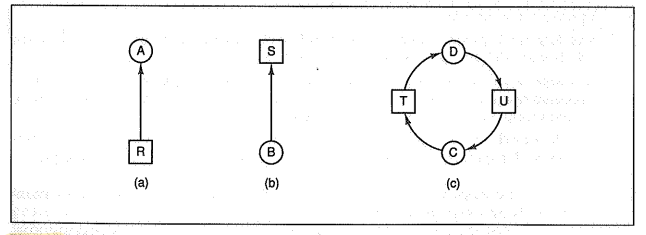
\includegraphics[width=0.6\linewidth]{assets/grafo9.png}
    \caption{Esempi di grafi di allocazione delle risorse. (a) acquisizione. (b) richiesta. (c) stallo.}
\end{figure}

\paragraph*{}
I grafi sono uno strumento utile a capire se una certa sequenza di richieste e rilasci porti o meno ad un deadlock.

Una prima soluzione che può venire in mente è quella di un esecuzione dei programmi sequenziale, in modo da troncare il problema alla radice.. tuttavia essa non è in generale una buona soluzione.

Normalmente per trattare adeguatamente le situazioni di stallo si possono impiegare quattro strategie:
\begin{itemize}
    \item \textbf{ignoramento del problema}, forse se tu lo ignori anche questo ti ignorerà.
    \item \textbf{rilevamento e risoluzione}: quando si verifica occorre scoprirlo e risolverlo.
    \item \textbf{evitamento}: cercare dinamicamente di evitare le situazioni di stallo con un'accorta politica di allocazione delle risorse.
    \item \textbf{prevenzione}: negare una delle quattro condizioni necessarie.
\end{itemize}

\paragraph*{}
\paragraph*{nota}
Esistono anche grafi con risorse multiple:
\begin{figure}[H]
    \centering
    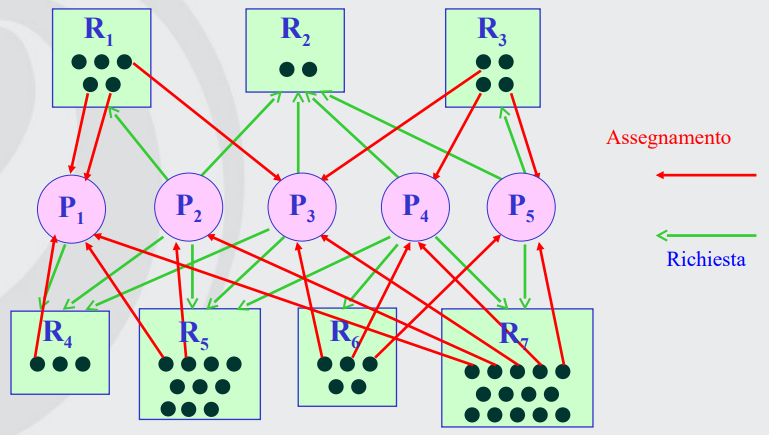
\includegraphics[width=0.8\linewidth]{assets/grafimultiple9.png}
    \caption{Esempi di grafi di allocazione delle risorse multiple.}
\end{figure}

\paragraph*{}
\section{L'algoritmo dello struzzo}
Pretendere semplicemente che il problema non esista.

Questo approccio è adottato dalla maggior parte dei sistemi operativi, tra cui UNIX e Windows. Questa scelta è presa in quanto gli utenti preferiscono una situazione di stallo occasionale ad una regola rigida che imponga l'utilizzo di singolo processo o file per utente..

\paragraph*{}
\section{Identificazione e risoluzione}
Il sistema in questo caso permette il verificarsi del deadlock, cerca di capire quando si verifica e agisce a riguardo.

\subsection{Identificazione con una risorsa per classe}
Supponiamo il caso più semplice: una risorsa per tipo.

Si costruisce un grafo tipo quello in figura \ref{grafi9}, se esiste un ciclo allora esiste un deadlock.

\begin{figure}[H]
    \centering
    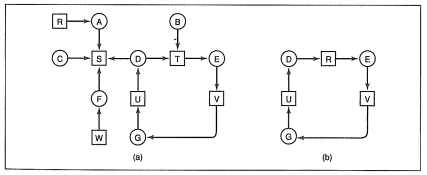
\includegraphics[width=0.6\linewidth]{assets/grafi9.png}
    \caption{(a) un grafo delle risorse. (b) un ciclo di (a).}
    \label{grafi9}
\end{figure}

L'algoritmo per l'identificazione considera a turno ogni nodo come radice di un albero, poi esegue una ricerca per ogni nodo sottostante e, se torna ad un nodo già incontrato allora ha identificato un ciclo. Non è uno dei migliori algoritmi ma è di facile comprensione.

\paragraph*{}
Nel caso di risorse singole un generico algoritmo richiede $n^2$ operazioni (n = numero di processi); Nel caso di risorse multiple $m*n^2$ operazioni (m = numero di tipi di risorse).

\subsection{Risoluzione}

\subsubsection{Con prerilascio}
In alcuni casi è possibile togliere una risorsa ad un processo ed assegnarla ad un altro. In molti casi è richiesto un intervento manuale. È una soluzione possibile in alcuni casi ma spesso difficile. 

\subsubsection{Con ritorno a stato precedente}
In questo caso si mettono dei \textbf{checkpoint} sui processi. Si scrive in un file lo stato delle risorse. Quando si scopre un deadlock si fa in modo che un processo torni ad uno stato precedente (\textit{rollback}) perdendo il lavoro svolto oltre. 

\subsubsection{Con eliminazione}
Il modo più semplice in assoluto prevede di eliminare processi finché non si esce dallo stallo. Si cerca ovviamente di eliminare quei processi il cui riavvio non è dannoso.

\section{Evitamento}
L'evitamento è possibile a patto di avere delle informazioni preliminari.

Si definisce uno stato del sistema, identificandolo come \textbf{sicuro} o \textbf{non sicuro}. In uno stato sicuro il sistema può garantire che tutti i processi avranno termine, in quello non sicuro non c'è alcuna garanzia. 


\begin{figure}[H]
    \centering
    \begin{subfigure}{.9\textwidth}
    \centering
      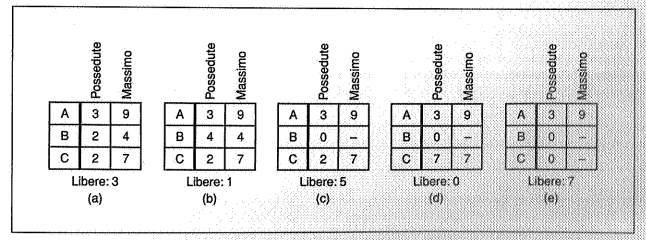
\includegraphics[width=1\linewidth]{assets/sicuro9.png}
      \caption{da (a) sicuro}
    \end{subfigure}
    \paragraph*{}
    \begin{subfigure}{.9\textwidth}
    \centering
      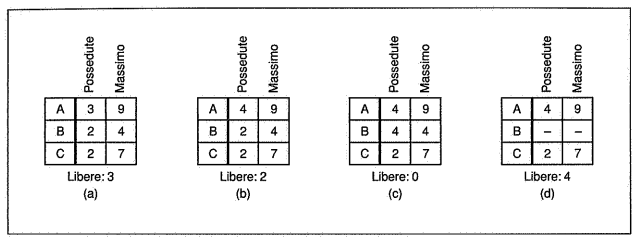
\includegraphics[width=1\linewidth]{assets/nonsicuro9.png}
      \caption{ da (b) non sicuro}
    \end{subfigure}
    \caption{Esempi di stati sicuri e non.}
\end{figure}

\subsection{L'algoritmo del banchiere per una singola risorsa}
Algoritmo di Dijkstra che permette di evitare situazioni di stallo. Prende spunto dalla maniera in cui un banchiere di una piccola città tratta un gruppo di clienti ai quali ha garantito delle linee di credito. Quello che l'algoritmo fa è controllare se il garantire una richiesta porti ad uno stato non sicuro e, se ciò accade, la richiesta viene rifiutata.

\begin{figure}[H]
    \centering
    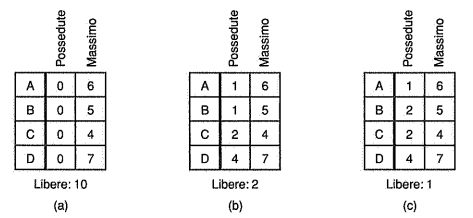
\includegraphics[width=0.6\linewidth]{assets/banchiere9.png}
    \caption{Tre stati di allocazione delle risorse: (a) sicuro. (b) sicuro. (c) non sicuro.}
\end{figure}

\paragraph*{}
\paragraph*{}
I clienti gestiscono i loro affari richiedendo di tanto in tanto dei prestiti. 

Se tutti i clienti richiedessero la cifra massima per i loro prestiti immediatamente il banchiere non potrebbe soddisfare nessuno di loro. 

Uno stato non sicuro non è detto che porti ad un deadlock.

L'algoritmo considera così ogni richiesta nel momento in cui essa si presenta, ed analizza se porta ad uno stato sicuro. Se lo fa esaurisce la richiesta, altrimenti viene posposta. Per verificare che lo stato successivo sia sicuro il banchiere controlla di avere abbastanza risorse per poter soddisfare le richieste di un cliente. Se tutti i prestiti possono essere restituiti lo stato è sicuro e la richiesta iniziale può essere soddisfatta.


\paragraph*{}
\subsection{L'algoritmo del banchiere per risorse multiple}
L'algoritmo appena visto può essere generalizzato a risorse multiple.

\begin{figure}[H]
    \centering
    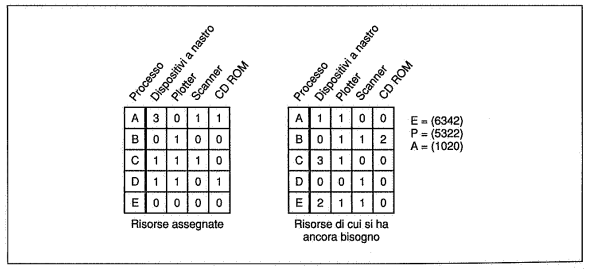
\includegraphics[width=0.6\linewidth]{assets/banchieremultiple9.png}
    \caption{L'algoritmo del banchiere con risorse multiple.}
\end{figure}

Si utilizzano due matrici, una per le risorse assegnate e una per quelle ancora necessarie. I tre vettori indicano le risorse esistenti (E), le risorse assegnate (P) e quelle disponibili (A).

L'algoritmo funziona in questo modo:
\begin{enumerate}
    \item Si cerca una riga in cui il numero di risorse ancora non richieste sono meno o altrettante di quelle di A. Se non esiste nessuna riga con questa caratteristica allora il sistema andrà in stallo.
    \item Si supponga che il processo della riga scelta richieda tutte le risorse di cui ha bisogno e finisca. Si marchi quindi il processo come terminato e si aggiungano ad A le risorse che esso deteneva.
    \item Si ripetano i due punti precedenti finché tutti i processi vengono marcati come completati o si identifichi uno stallo, alla fine si può marcare lo stato iniziale come sicuro o non sicuro.
\end{enumerate}

\paragraph*{}
Anche in questo caso i processi devono comunicare in anticipo il loro fabbisogno globale, in modo che il sistema possa calcolare la seconda matrice in ogni istante. Questo fatto rende praticamente inutilizzabile questa strategia, quasi mai accade che i processi conoscano in anticipo il massimo numero di risorse di cui hanno bisogno per completarsi.


\paragraph*{}
\section{Prevenzione}
Se si potesse garantire che almeno una delle condizioni che permettono l'esistenza del deadlock non sarà mai verificata, allora non si avrebbero mai situazioni di stallo.

\subsection{Negazione della condizione di mutua esclusione}
Se nessuna risorsa fosse mai assegnata in maniera esclusiva ad un unico processo non avremmo stalli.

Un possibile approccio è lo \textbf{spooling}: occorre un processo demone e una directory di spooling, il demone è l'unico a richiedere la risorsa, i processi normali usano la directory per chiedere al demone di usare la risorsa sui file che vi inseriscono. (\textit{e.g.: stampa, posta elettronica..}).

Sfortunatamente questo approccio non è sempre utilizzabile. L'unica cosa che possiamo fare sempre è evitare di assegnare una risorsa se non è strettamente necessario, ed assicurarci che il minor numero possibile di processi abbiano bisogno di quella risorsa.


\subsection{Negazione della condizione hold-and-wait}
Un modo per ottenere quanto richiesto è obbligare i processi a richiedere tutte le risorse di cui hanno bisogno prima di iniziare l'esecuzione, andando in attesa nel caso ne manchi qualcuna.

Un primo problema di questa strategia è lo stesso dell'algoritmo del banchiere: i processi non sanno in anticipo le risorse di cui avranno bisogno. Un secondo problema aggiuntivo invece è la poca efficienza nell'utilizzo delle risorse, esse saranno occupate per tutto il tempo dell'esecuzione di un processo anche se utilizzate per un breve istante.

\paragraph*{}
Una tecnica alternativa per implementare la strategia prevede che un processo prima di richiedere una nuova risorsa rilasci temporaneamente tutte quelle che possiede, per poi richiederle tutte insieme, aggiungendo quella nuova.


\subsection{Negazione della condizione di mancanza di prerilascio}
Questa strategia risulta meno promettente della seconda, praticamente impossibile da realizzare nella maggior parte dei casi.


\subsection{Negazione della condizione di attesa circolare}
Ci sono diversi modi di eliminare l'attesa circolare. Il più sensato è quello di numerare globalmente tutte le risorse presenti, permettendo poi ai processi di richiedere le risorse quando vogliono, ma seguendo l'ordine numerico. Utilizzando questa regola il grafo non può contenere cicli.

La pecca di questa soluzione è la difficoltà nel trovare un ordinamento che soddisfi tutti.

\paragraph*{}
\section{Starvation}
Un problema strettamente legato ai deadlock è la \textbf{starvation}\footnote{\textit{starvation sarebbe "morire d'inedia"}}: una cattiva politica di gestione delle risorse può far si che alcuni processi non vengano mai serviti, pur non essendo in stallo. 

Un semplice modo per evitarla è usare una politica \textbf{FIFO}.

Un altro modo potrebbe essere offrire una percentuale della risorsa adeguata ad ogni processo.

Un altro ancora sarebbe aumentare la priorità di un processo in coda da molto.